\documentclass{article}
	\usepackage{tikz}
	\usetikzlibrary{calc, graphs, positioning, shapes.misc}
	\definecolor{col0}{RGB}{255, 51, 51}
	\definecolor{col1}{RGB}{215,255, 51}
	\definecolor{col2}{RGB}{ 51,255,133}
	\definecolor{col3}{RGB}{ 51,133,255}
	\definecolor{col4}{RGB}{215, 51,255}

\begin{document}
% \resizebox{200}{!}
% {
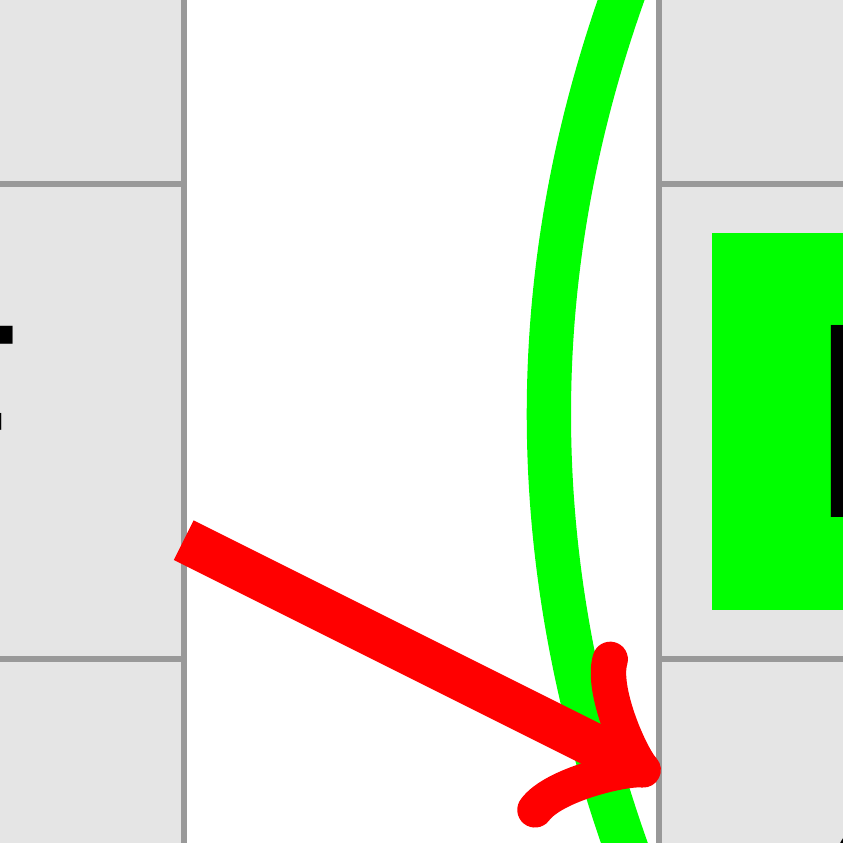
\begin{tikzpicture}
	[
		node distance=0mm,
		box/.style={
				rectangle,
				minimum size=6mm,
				ultra thin,
				draw=black!40,
				fill=black!10,
			},
		emptyBox/.style={
				rectangle,
				minimum height=18mm,
				minimum width=6mm,
				ultra thin,
				draw=black!40,
				fill=white,
			},
	]
	\useasboundingbox (-5,-5) rectangle (5,5);
	\begin{scope}[transform canvas={scale=10}]
	\matrix[row sep=0mm,column sep=0mm, every node/.style=box] {
		\node (n6) {}; & \node (n7) {}; & \node (n8)  {}; \\
		\node (n5) {}; &                & \node (n9)  {}; \\
		\node (n4) {}; &                & \node (n10) {}; \\
		\node (n3) {}; &                & \node (n11) {}; \\
		\node (n2) {}; & \node (n1) {}; & \node (n12) {}; \\
	};
	\node [emptyBox, below= of n7 ] {};

	\begin{scope}[font=\sffamily]
		\node at (n1)  [] {D};
		\node at (n2)  [] {};
		\node at (n3)  [] {};
		\node at (n4)  [] {F};
		\node at (n5)  [] {};
		\node at (n6)  [red] {G};
		\node at (n7)  [] {};
		\node at (n8)  [fill=red] {A};
		\node at (n9)  [] {};
		\node at (n10) [fill=green] {B};
		\node at (n11) [] {C};
		\node at (n12) [] {};
		\draw [->, green, ultra thick] (n12) to [bend left] (n8);
		\draw [->, red, ultra thick, bend right] (n4) -- (n11);
	\end{scope}
	\end{scope}
\end{tikzpicture}


\end{document}